%!TEX program = xelatex
%!TEX root = ./thesis.tex
\section{Target Environments}\label{sec_env}
\subsection{Summary of environment design}
We propose and develop a set of tasks that are representatives of deep reinforcement learning environments with continuous action space, multi-modal state space and sparse reward functions. The design of the robot physical systems are based on the 3D robot environments~\cite{roboschool_2018} in OpenAI Gym~\cite{openaigym}. The external environments and reward functions of the target tasks are different from the original environments in OpenAI Gym. There are three classes of 3D robot agents in the environments OpenAI Gym: Ant, Humanoid and Swimmer. The "Ant" agent is a quadruped robot with 8-dimensional action space, the "Humanoid" agent is a humanoid robot with 16-dimensional action space, and the "Swimmer" agent is a worm-like robot with 2-dimensinoal action space.  The three agents are showed in Figure~\ref{fig_agent_ant}, Figure~\ref{fig_agent_humanoid} and Figure~\ref{fig_agent_swimmer}.

We mainly focus on different tasks based on the "Ant" agent, because the agent has the capability of solving a rich variety of high-level tasks, while the learning of agent's basic control skills are reasonably but not too challenging. 
Compared to the "Ant" agent, the "Swimmer" agent is too simple and its capability of solving hierarchical tasks is limited. The "Humanoid" agent's on the other hand, is much more unstable physical system compared to "Ant", and poses too much difficulty on its basic locomotion skills.
\begin{figure}[H]
	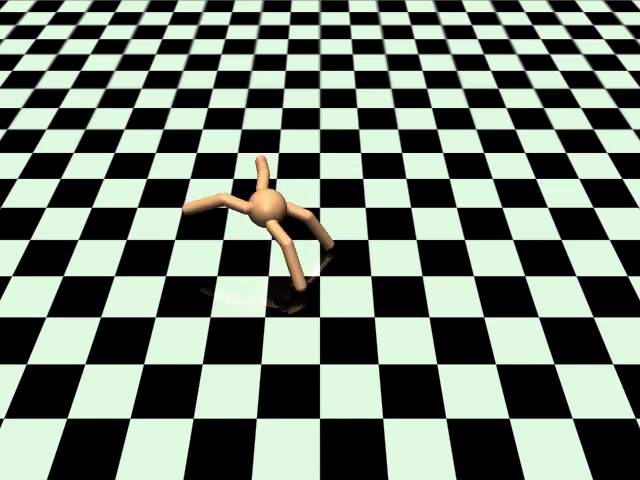
\includegraphics[width=0.5\textwidth]{images/agent_ant.png}
	\centering
	\caption{The "Ant" agent}\label{fig_agent_ant}
\end{figure}

\begin{figure}[H]
	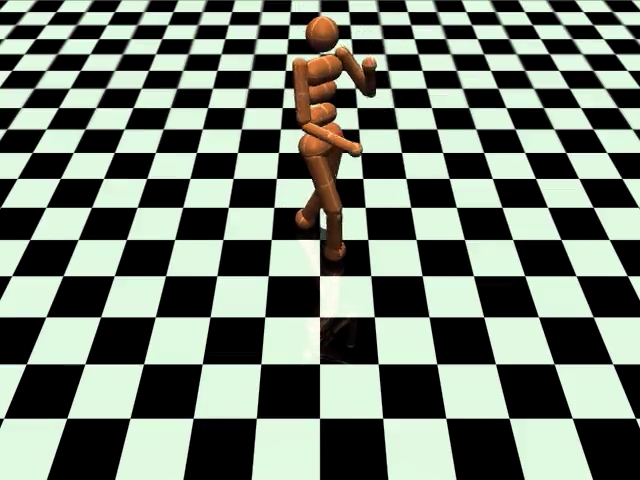
\includegraphics[width=0.5\textwidth]{images/agent_humanoid.png}
	\centering
	\caption{The "Humanoid" agent}\label{fig_agent_humanoid}
\end{figure}
\begin{figure}[H]
	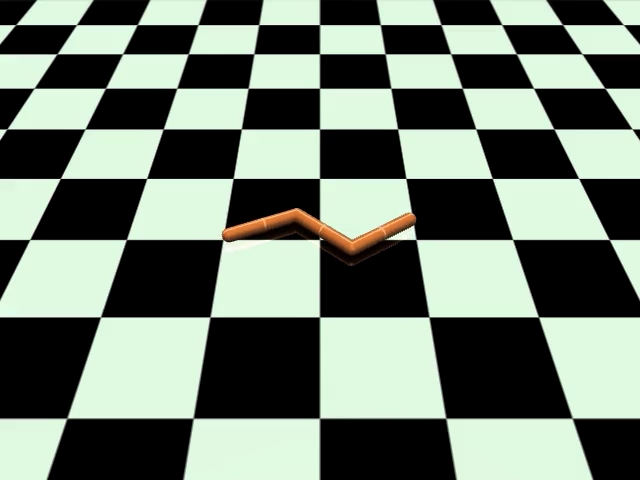
\includegraphics[width=0.5\textwidth]{images/agent_swimmer.png}
	\centering
	\caption{The "Swimmer" agent}\label{fig_agent_swimmer}
\end{figure}
%To provide a consistent comparison with other studies, the development of 
%!TEX program = xelatex
%!TEX root = ./thesis.tex

\subsection{Detailed Environment Specifications}
We provide a detailed description of the experiment environments in this section. All of the environments are based on the Ant task~\cite{openaigym}. 

In the original Ant task, the agent receives a 111-dimensional motion sensor input and produces an 8-dimensional action output. The input consists of a 13-dimensional vector that contains the robot's pose information, a 14-dimensional vector that represents its velocity information, and an 84-dimensional vector that contains contact force information. However, information about the agent's absolute position in the world map is not available.

For the proposed environments, the agent receives not only the 111-dimensional motion sensor input, but also a $64\times 64\times 1$ dimensional grayscale image observation. A sample image observation is shown in Figure~\ref{fig_ant_imgobs}. The image is not in a high resolution but is sufficient for the agent to observe the necessary information for the proposed tasks.

\begin{figure}[H]
	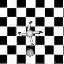
\includegraphics{images/ant_imgobs.png}
	\centering
	\caption{A sample image observation of the target environments}
\end{figure}\label{fig_ant_imgobs}

A basic task, namely move0, is similar to the Ant environment in OpenAI Gym~\cite{openaigym}. The difference is that the state space has an extra image input. The agent is required to move in a specific direction $g_0=(1,0)$, and the reward at each time-step is given by:
\begin{align}
r = v_g + 1-c_p-c_c
\end{align}
where $v_g=v \cdot g_0$ is the forward reward, which rewards the agent for moving in the target direction. A spherical object presents in the environments at a constant distance from the robot agent to represent the target direction.  $c_p$ is the control cost, which is the power that the agent is consuming, and $c_c$ is the contact cost, which penalizes the agent for collisions. The episode terminates when the agent enters the unrecoverable state of being upside-down, or if the episode length reaches 1000 time-steps.

Apart from move0, a set of similar tasks with different target directions are denoted as move1, move2, move3, ..., move7. These tasks are similar to move0 because the goal direction is different. The image observation is actually redundant for all these low-level tasks, because the agent only needs to move in one specific direction in their corresponding environments. Snapshots of these source tasks are shown in Figure~\ref{fig:task8}.
\begin{figure}[!htbp]
	\centering
	\begin{subfigure}[t]{0.3\textwidth}
		\centering
		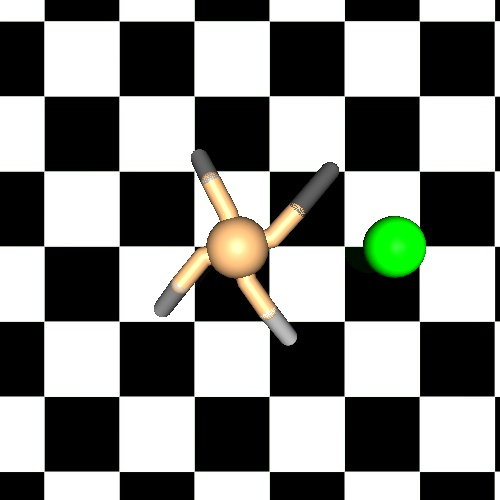
\includegraphics[width=\textwidth]{move0}
		\caption{move0}
	\end{subfigure}%
	~ 
	\begin{subfigure}[t]{0.3\textwidth}
		\centering
		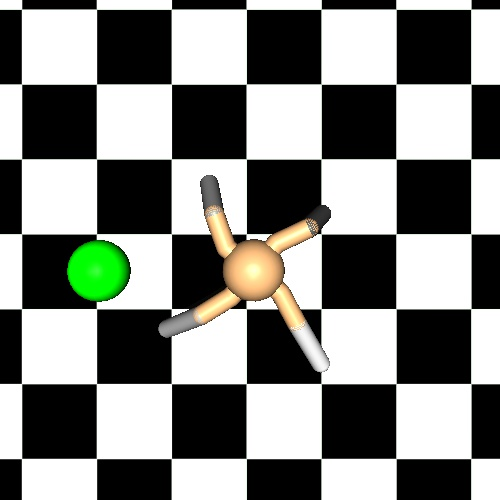
\includegraphics[width=\textwidth]{move1}
		\caption{move1}
	\end{subfigure}
	~ 
	\begin{subfigure}[t]{0.3\textwidth}
		\centering
		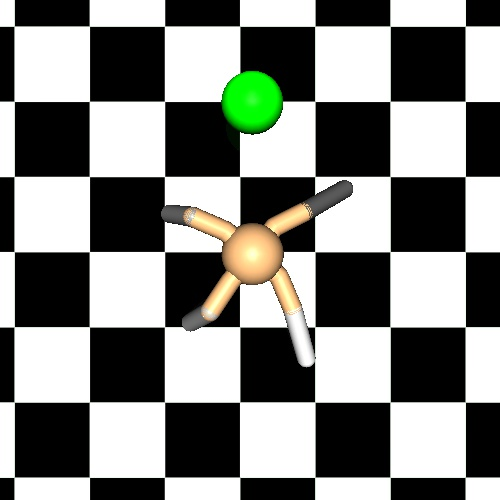
\includegraphics[width=\textwidth]{move2}
		\caption{move2}
	\end{subfigure}
	~ 
	\begin{subfigure}[t]{0.3\textwidth}
		\centering
		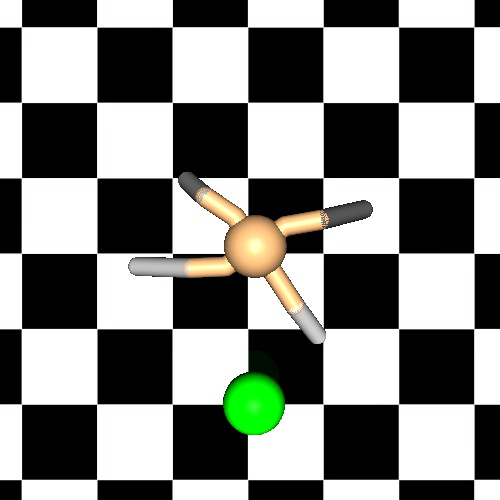
\includegraphics[width=\textwidth]{move3}
		\caption{move3}
	\end{subfigure}
	~ 
	\begin{subfigure}[t]{0.3\textwidth}
		\centering
		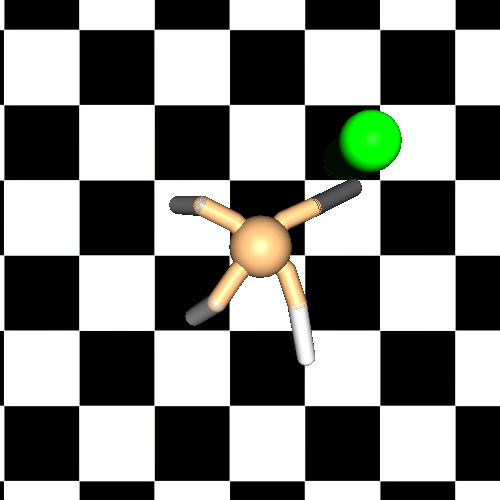
\includegraphics[width=\textwidth]{move4}
		\caption{move4}
	\end{subfigure}
	~ 
	\begin{subfigure}[t]{0.3\textwidth}
		\centering
		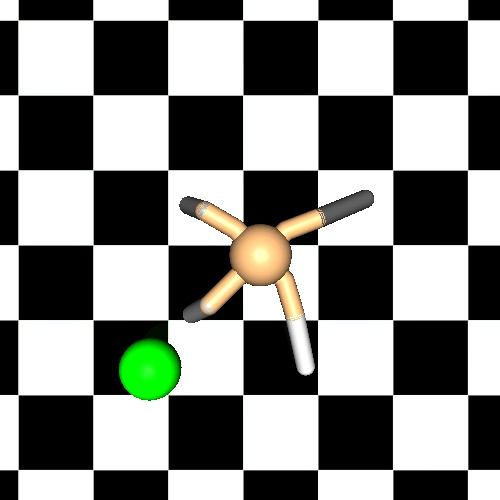
\includegraphics[width=\textwidth]{move5}
		\caption{move5}
	\end{subfigure}
	~ 
	\begin{subfigure}[t]{0.3\textwidth}
		\centering
		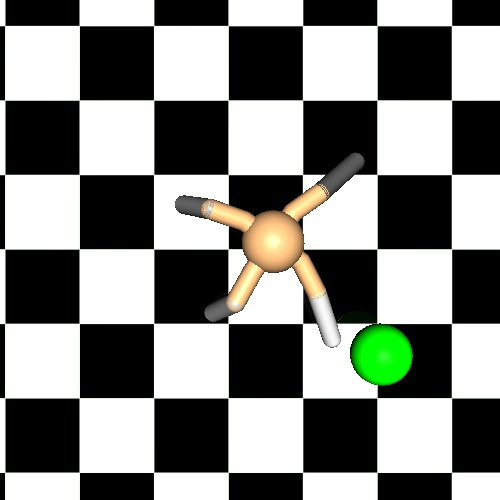
\includegraphics[width=\textwidth]{move6}
		\caption{move6}
	\end{subfigure}
	~ 
	\begin{subfigure}[t]{0.3\textwidth}
		\centering
		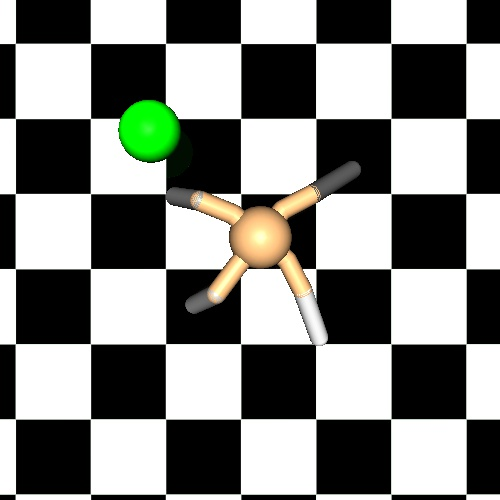
\includegraphics[width=\textwidth]{move7}
		\caption{move7}
	\end{subfigure}

	\caption{The source tasks}
	\label{fig:task8}
\end{figure}

Apart from these simple task, we also propose a set of tasks with more complexity. We propose several tasks with multi-modal state spaces such as moveg2, movecont, dynamicg8. These tasks require the agent to learn not only from the state representation but also the image representation. We also propose several more challenging tasks which has sparse reward fucntions, such as reachcont. The agent receives sparse reward signals in these environments. The target direction or location is represented by a spherical object and can be seen in the image observation.
The set of all the proposed environments are described in details in table \ref{table_ant_envs}.


\begin{table}[!htbp]

\begin{center}
\begin{tabular}{|c|p{3cm}|p{4cm}|p{4cm}|}
\hline
Task name & Goal & Reward  &  Description \\
\hline\hline
move0 & velocity: $g_0=(1,0)$ &$ v_g+1-c_p-c_c$  & move in a target direction \\
\hline
move1 & velocity: $g_1=(-1,0)$ &$ v_g+1-c_p-c_c$  & move in a target direction\\
\hline
move2 & velocity: $g_2=(0,1)$ &$ v_g+1-c_p-c_c$  & move in a target direction \\
\hline
move3 & velocity: $g_3=(0,-1)$ &$ v_g+1-c_p-c_c$  & move in a target direction \\ 
\hline 
move4 & velocity: $g_4=(\sqrt{2}/2,\sqrt{2}/2)$ &$ v_g+1-c_p-c_c$  & move in a target direction \\ 
\hline 
move5 & velocity: $g_5=(-\sqrt{2}/2,-\sqrt{2}/2)$ &$ v_g+1-c_p-c_c$  & move in a target direction \\ 
\hline 
move6 & velocity: $g_6=(\sqrt{2}/2,-\sqrt{2}/2)$ &$ v_g+1-c_p-c_c$  & move in a target direction \\ 
\hline 
move7 & velocity: $g_7=(-\sqrt{2}/2,\sqrt{2}/2)$ &$ v_g+1-c_p-c_c$  & move in a target direction \\ 
\hline 
moveg2 & velocity samples from: $\{g_0,g_1\}$ &$ v_g+1-c_p-c_c$  & each episode has a random sampled target direction \\ \hline
%moveg4 & velocity samples from: $\{g_0,g_1,g_2,g_3\}$ &$ v_g+1-c_p-c_c$  & each episode has a random sampled target direction \\ \hline
%moveg8 & velocity samples from: $\{g_0,g_1, \dots,g_7\}$ &$ v_g+1-c_p-c_c$  & each episode has a random sampled target direction \\ \hline
movecont & velocity samples from the unit circle&$ v_g+1-c_p-c_c$  & each episode has a random sampled target direction \\ \hline
dynamicg8 &  velocity samples from: $\{g_0,g_1, \dots,g_7\}$ &$ v_g$  & the target direction is re-sampled with probability 0.005 at each time-step  \\ \hline
%dynamiccont & velocity samples from a continuous range of all unit directions &$ v_g$  & the target direction is re-sampled with probability 0.005 at each time-step  \\ \hline
%reachg4 & position samples from $\{g_0,g_1,g_2,g_3\}$ & $I(\lVert x-g\rVert_2^2<0.5) - 0.01$  & The agent is terminated when reaching a target position\\ \hline
reachcont & position samples from the unit circle & $I(\lVert x-g\rVert_2^2<0.5) - 0.01$  & the episode is terminated when reaching a target position\\ \hline
reachcontreg & position samples from the unit circle & $5I(\lVert x-g\rVert_2^2<0.5) - 0.01$  & a new target is sampled and the episode continuous once the target position is reached\\ \hline
constdirreachreg & target direction samples from: $\{g_0,g_1, \dots,g_7\}$ & $5I(x_g > 1) - 0.01$  & a reward is given once the agent has moved in the target direction for a constant distance, then a new target is sampled\\ \hline
\end{tabular}
\end{center}
 \caption{Specification of the tasks}
\end{table}\label{table_ant_envs}



